\chapter{   Computer Vision}
% CHAPTER SETTINGS
\graphicspath{{./images/computer_vision/}}

\section{Edge Detection}

%%%%%%%%%%%%%%%%%%%%%%%%%%%%%%%%%%%%%%%%%%%%%%%%%%%%%%%%%%%%%%%%%%%%%%%%%%%%%%%%%%%%%%%%%%%%%%%%%%%%

\subsection{Describe canny detection algorithm?}
Here are the steps, which are needed to implement canny edge detection algorithm:
\begin{enumerate}
    \item Grayscale conversion
    \item Gaussian Blur
    \item Determine the Intensity Gradients
    \item Non Maximum Suppression
    \item Double Thresholding
    \item Edge Tracking by Hysteresis
\end{enumerate}

\subsubsection{Step 1: Convert the image to grayscale}
Convert 3 channels into 1.

\begin{figure}[!htb]
    \centering
    \begin{minipage}{.5\textwidth}
        \centering
        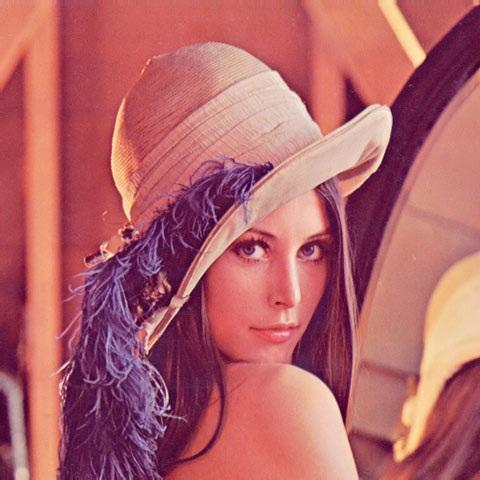
\includegraphics[width=40mm]{canny_original.jpg}
        \caption{Original}
    \end{minipage}%
    \begin{minipage}{.5\textwidth}
        \centering
        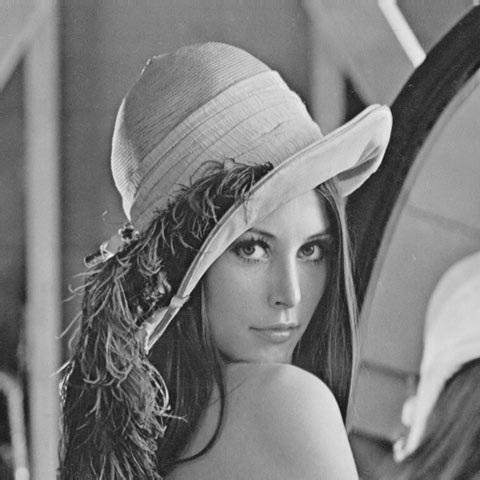
\includegraphics[width=40mm]{canny_grayscale.jpg}
        \caption{Grayscaled}
    \end{minipage}
\end{figure}


\subsubsection{Step 2: Apply Gaussian filter to smooth the image in order to remove the noise}
Since all edge detection results are easily affected by image noise, it is essential to filter out the noise to prevent false detection caused by noise. To smooth the image, a Gaussian filter is applied to convolve with the image.

\begin{figure}[!htb]
    \centering
    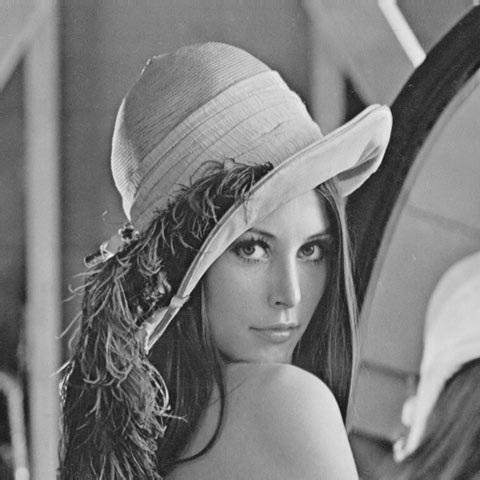
\includegraphics[width=40mm]{canny_grayscale.jpg}
    \caption{Gaussian blurred}
\end{figure}


\subsubsection{Step 3: Find the intensity gradients of the image}
An edge in an image may point in a variety of directions, so the Canny algorithm uses four filters to detect horizontal, vertical and diagonal edges in the blurred image. The edge detection operator (such as Roberts, Prewitt, or Sobel) returns a value for the first derivative in the horizontal direction ($G_{x}$) and the vertical direction ($G_{y}$). From this the edge gradient and direction can be determined. Here is an example of the sobel operator:

\begin{figure}[!htb]
    \centering
    \begin{minipage}{.5\textwidth}
        \centering
        $G_{x} = S_{x} * A =
        \left[ \begin{array}{rrrr}
        1 & 0 & -1 \\
        2 & 0 & -2 \\
        1 & 0 & -1 \\
        \end{array}\right] $
    \end{minipage}%
    \begin{minipage}{.5\textwidth}
        \centering
        $G_{y} = S_{y} * A =
        \left[ \begin{array}{rrrr}
        1 & 2 & 1 \\
        0 & 0 & 0 \\
        -1 & -2 & -1 \\
        \end{array}\right] $
    \end{minipage}
\end{figure}

\vspace{5mm}
\noindent Using the two operators you can then calculate the magnitude and the directional gradients of the image as follows:

\begin{figure}[!htb]
    \centering
    \begin{minipage}{.5\textwidth}
        \centering
        $|G| = \sqrt(G^{2}_{x} + G^{2}_{y})$
        \caption{Magnitude}
    \end{minipage}%
    \begin{minipage}{.5\textwidth}
        \centering
        $\Theta = arctan(G_{x}/G_{y})$
        \caption{Directinal gradients}
    \end{minipage}
\end{figure}

\vspace{5mm}
\noindent The resulting magnitude looks like:
\begin{figure}[!htb]
    \centering
    \begin{minipage}{.33\textwidth}
        \centering
        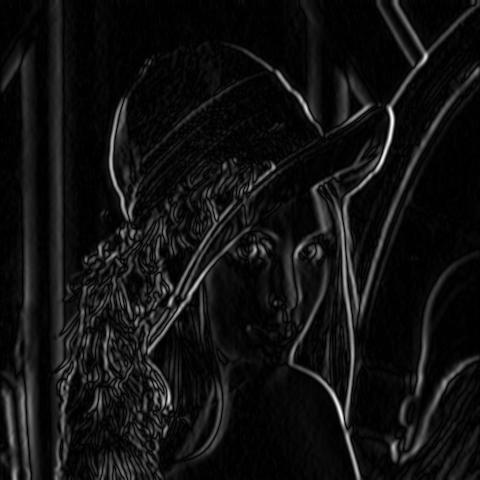
\includegraphics[width=40mm]{canny_sobel_x.jpg}
        \caption{$Sobel_{x}$}
    \end{minipage}%
    \begin{minipage}{.33\textwidth}
        \centering
        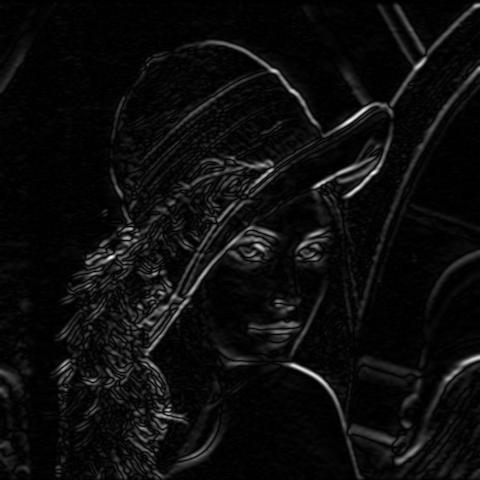
\includegraphics[width=40mm]{canny_sobel_y.jpg}
        \caption{$Sobel_{y}$}
    \end{minipage}
    \begin{minipage}{.33\textwidth}
        \centering
        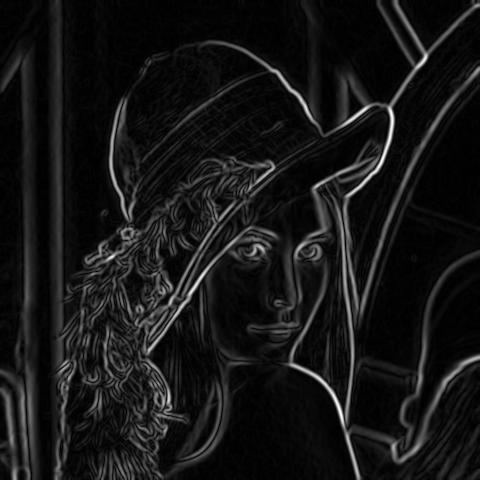
\includegraphics[width=40mm]{canny_magnitude.jpg}
        \caption{$Magnitude$}
    \end{minipage}
\end{figure}


\subsubsection{Step 4: Apply non-maximum suppression to get rid of spurious response to edge detection}
Non-maximum suppression is an edge thinning technique. After applying gradient calculation, the edge extracted from the gradient value is still quite blurred. Ideally, the final image should have only thin edges. Thus non-maximum suppression can help to suppress all the gradient values (by setting them to 0) except the local maxima, which indicate locations with the sharpest change of intensity value. The algorithm for each pixel in the gradient image is:

\begin{figure}[!htb]
    \centering
    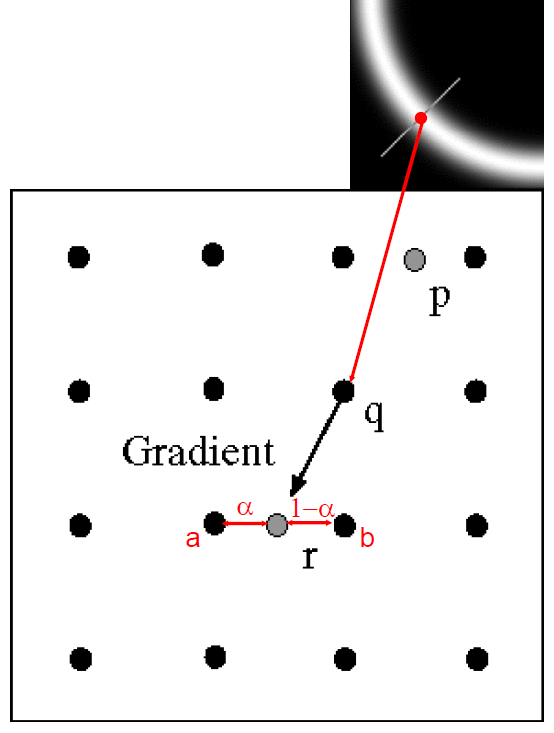
\includegraphics[width=40mm]{canny_nms_example.png}
\end{figure}


\noindent Non maximum suppression works by finding the pixel with the maximum value in an edge. In the above image, it occurs when pixel q has an intensity that is larger than both p and r where pixels p and r are the pixels in the gradient direction of q. If this condition is true, then we keep the pixel, otherwise we set the pixel to zero (make it a black pixel). Non maximum suppression can be achieved by interpolating the pixels for greater accuracy:

\begin{figure}[!htb]
    \centering
    $r = \alpha * b + (1 − \alpha) * a$
\end{figure}

\vspace{5mm}
\noindent Here is a resulting image:
\begin{figure}[!htb]
    \centering
    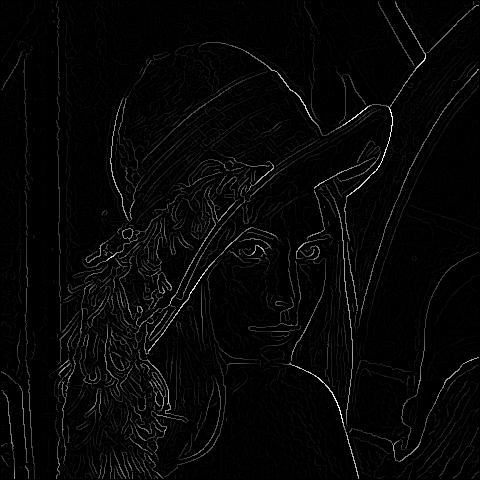
\includegraphics[width=45mm]{canny_nms.jpg}
    \caption{Non maximum suppression}
\end{figure}


\subsubsection{Step 5: Apply double threshold to determine potential edges}
After application of non-maximum suppression, remaining edge pixels provide a more accurate representation of real edges in an image. However, some edge pixels remain that are caused by noise and color variation. In order to account for these spurious responses, it is essential to filter out edge pixels with a weak gradient value and preserve edge pixels with a high gradient value. This is accomplished by selecting high and low threshold values. If an edge pixel’s gradient value is higher than the high threshold value, it is marked as a strong edge pixel. If an edge pixel’s gradient value is smaller than the high threshold value and larger than the low threshold value, it is marked as a weak edge pixel. If an edge pixel's value is smaller than the low threshold value, it will be suppressed. The two threshold values are empirically determined and their definition will depend on the content of a given input image.

\begin{figure}[!htb]
    \centering
    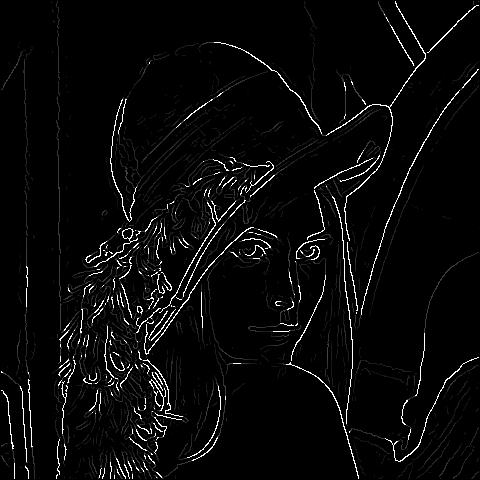
\includegraphics[width=40mm]{canny_double_thresholding.jpg}
    \caption{Double thresholding}
\end{figure}


\subsubsection{Step 6: Track edge by hysteresis: Finalize the detection of edges by suppressing all the other edges that are weak and not connected to strong edges}
So far, the strong edge pixels should certainly be involved in the final edge image, as they are extracted from the true edges in the image. However, there will be some debate on the weak edge pixels, as these pixels can either be extracted from the true edge, or the noise/colour variations. To achieve an accurate result, the weak edges caused by the latter reasons should be removed. Usually a weak edge pixel caused from true edges will be connected to a strong edge pixel while noise responses are unconnected. To track the edge connection, blob analysis is applied by looking at a weak edge pixel and its 8-connected neighbourhood pixels. As long as there is one strong edge pixel that is involved in the blob, that weak edge point can be identified as one that should be preserved.

\begin{figure}[!htb]
    \centering
    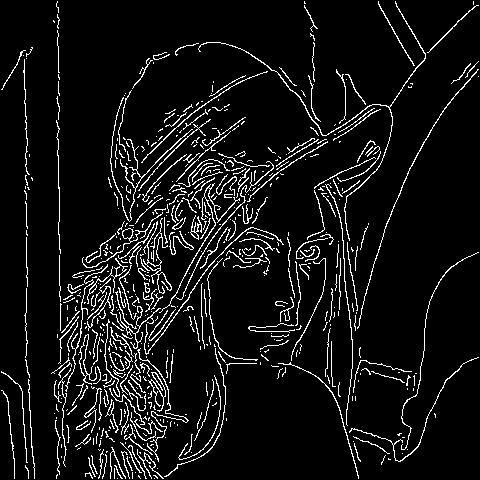
\includegraphics[width=40mm]{canny_final.jpg}
    \caption{Final Result from Canny Edge Detection Algorithm}
\end{figure}

%%%%%%%%%%%%%%%%%%%%%%%%%%%%%%%%%%%%%%%%%%%%%%%%%%%%%%%%%%%%%%%%%%%%%%%%%%%%%%%%%%%%%%%%%%%%%%%%%%%%



% Drawbacks of canny edge detector
% While traditional Canny edge detection provides relatively simple but precise methodology for edge detection problem, with more demanding requirements on the accuracy and robustness on the detection, the traditional algorithm can no longer handle the challenging edge detection task. The main defects of the traditional algorithm can be summarized as follows:
%
% 1. A Gaussian filter is applied to smooth out the noise, but it will also smooth the edge, which is considered as the high frequency feature. This will increase the possibility of missing weak edges, and the appearance of isolated edges in the result.
%
% As both edge and noise will be identified as high frequency signal, simple Gaussian filter will add smooth effect on both of them. However, in order to reach high accuracy of detection of the real edge, it is expected that more smooth effect should be added to noise and less smooth effect should be added to the edge. Bing Wang and Shaosheng Fan from Changsha University of Science and Technology developed an adaptive filter, where the filter will evaluate discontinuity between greyscale values of each pixel.[8] The higher the discontinuity, the lower the weight value is set for the smooth filter at that point. Contrarily, the lower the discontinuity between the greyscale values, the higher the weight value is set to the filter.
%
% 2. For the gradient amplitude calculation, the old Canny edge detection algorithm uses the Centre in a small 2×2 neighbourhood window to calculate the finite difference mean value to represent the gradient amplitude. This method is sensitive to noise and can easily detect false edges and lose real edges.
%
% The gradient magnitude and direction can be calculated with a variety of different edge detection operators, and the choice of operator can influence the quality of results. A very commonly chosen one is the 3x3 Sobel filter. However, other filters may be better by, such as a 5x5 Sobel filter which will reduce noise or the Scharr filter which has better rotational symmetry. Other common choices are Prewitt (used by Zhou [10]) and Roberts Cross.
%
% 3. In the traditional Canny edge detection algorithm, there will be two fixed global threshold values to filter out the false edges. However, as the image gets complex, different local areas will need very different threshold values to accurately find the real edges. In addition, the global threshold values are determined manually through experiments in the traditional method, which leads to complexity of calculation when a large number of different images need to be dealt with.
%
% In order to resolve the challenges where it is hard to determine the dual-threshold value empirically, Otsu's method [11] can be used on the non-maximum suppressed gradient magnitude image to generate the high threshold. The low threshold is typically set to 1/2 of the high threshold in this case. Since the gradient magnitude image is continuous-valued without a well-defined maximum, Otsu's method has to be adapted to use value/count pairs instead of a complete histogram.
%
% 4.The result of the traditional detection cannot reach a satisfactory high accuracy of single response for each edge - multi-point responses will appear.
%
% While the traditional canny edge detection have implemented a good detection result to meet with the first two criteria, it does not meet with the single response per edge strictly. A mathematical morphology to thin the detected edge is developed by Mallat S and Zhong.[9]


% >> add links for the papers
% https://en.wikipedia.org/wiki/Canny_edge_detector



%
% Info: What is blob analysis?
% Connected-component labelling  is an algorithmic application of graph theory, where subsets of connected components are uniquely labelled based on a given heuristic.

% get here the question about operators
